\documentclass[notes]{beamer}
\usepackage{etex}
\usepackage{pgf}
\usepackage{color}
\definecolor{lblue}{rgb}{0.5,0.5,1}
\usepackage{xspace}
\usepackage{listings}
\usepackage{adjustbox}
\usepackage{spverbatim}
\usepackage{subcaption}
\usepackage{textpos}
\usepackage{etoolbox}
\usepackage{xparse}
\usepackage[shadow , roundedcorners, customcolors, getthemecolors]{dynblocks}

\usepackage{tikz}
\usepackage{tikz-qtree}
\usetikzlibrary{shapes,arrows,positioning,shadows,trees,shadows.blur}
\usepackage{pgfplots}
\usepackage{filecontents}
\usepackage{rotating}
\usepackage{graphicx}

\mode<presentation>
{
	%\setbeamertemplate{footline}[page number]
	\setbeamertemplate{footline}{%
  \raisebox{2pt}{\makebox[\paperwidth]{\hfill\makebox[20pt]{\textcolor{gray}{\insertframenumber/\inserttotalframenumber}}}}}
  \usetheme{Goettingen}
	%\usecolortheme{dove}
  \setbeamercovered{transparent}
}


\usepackage[english]{babel}
% or whatever

\usepackage[latin1]{inputenc}
% or whatever

\usepackage{times}
\usepackage[T1]{fontenc}
% Or whatever. Note that the encoding and the font should match. If T1
% does not look nice, try deleting the line with the fontenc.

\newcommand{\parspace}{}
%\newcommand{\parspace}{\vspace{-\baselineskip}}
\newcommand{\NN}{\mathbb{N}}
\newcommand{\PP}{\mathbb{P}}
\newcommand{\ZZ}{\mathbb{Z}}
\newcommand{\FF}{\mathbb{F}}           %% for finite fields
\newcommand{\GG}{\mathbb{G}}

\newcommand{\Zrq}{\mathbb{Z}^\ast_q}
\newcommand{\ZN}{\mathbb{Z}_N}

\newcommand{\cA}{\ensuremath{\mathcal{A}}\xspace}
\newcommand{\cB}{\ensuremath{\mathcal{B}}\xspace}
\newcommand{\cC}{\mathcal{C}}
\newcommand{\cD}{\mathcal{D}}
\newcommand{\cE}{\mathcal{E}}
\newcommand{\cF}{\mathcal{F}}
\newcommand{\cG}{\mathcal{G}}
\newcommand{\cH}{\mathcal{H}}
\newcommand{\cI}{\mathcal{I}}
\newcommand{\cK}{\mathcal{K}}
\newcommand{\cL}{\mathcal{L}}
\newcommand{\cM}{\mathcal{M}}
\newcommand{\cO}{\mathcal{O}}
\newcommand{\cP}{\mathcal{P}}
\newcommand{\cQ}{\mathcal{Q}}
\newcommand{\cR}{\mathcal{R}}
\newcommand{\cS}{\mathcal{S}}
\newcommand{\cT}{\mathcal{T}}
\newcommand{\cU}{\mathcal{U}}
\newcommand{\cX}{\mathcal{X}}

\newcommand{\secpar}{\lambda{}}

% assigment, random-choice, etc.
\newcommand{\asgn}{:=}          % assigment \sigma := (a,b,c)
\newcommand{\algout}{\gets}     % algorithm output (sk,pk) <-- KGen(...), hash- and pr-functions too
\newcommand{\ralgout}{\stackrel{R}{\gets}}     % output of random algorithm
\newcommand{\cmp}{=}            % comparison a = b
\newcommand{\rch}{\in_R}        % random choice x \in_R {0,1}^m

\newcommand{\bits}{\{0,1\}}
\newcommand{\rin}{\in_R}
\newcommand{\rinb}{\rin\bits}
\newcommand{\concat}{\!\parallel\!}
%\newcommand{\bitlength}[1]{\lvert{#1}\rvert_{_2}}

\DeclareMathOperator{\ord}{ord}
\DeclareMathOperator{\mymod}{mod}
\newcommand{\MYMOD}[1]{\;(\mymod {#1})}
\DeclareMathOperator{\lcm}{lcm}
\DeclareMathOperator{\dom}{dom}
\newcommand{\legen}[2]{\bigl(\tfrac{#1}{#2}\bigr)}
\newcommand{\jacob}[2]{\bigl(\tfrac{#1}{#2}\bigr)}

\newcommand{\writtenby}[1]{~\mbox{\normalsize\normalfont{(#1)}}}

% new commands
\newcommand{\pwd}{\mathrm{pw}}
\newcommand{\pwdv}{\ensuremath{\mathbf{pw}}}
\newcommand{\msg}{\mathrm{m}}
\newcommand{\mout}{m_{\mathrm{out}}}
\renewcommand{\min}{m_{\mathrm{in}}}
\newcommand{\pake}{\mathrm{PAKE}}
\newcommand{\iencode}{\ensuremath{\mathtt{iEncode}}\xspace}
\newcommand{\idecode}{\ensuremath{\mathtt{iDecode}}\xspace}
\newcommand{\ihme}{\mathrm{IHME}}
\newcommand{\IHME}{\mathtt{IHME}}
\newcommand{\map}{\mathtt{map}}
\newcommand{\mapinv}{\mathtt{mapinv}}
\newcommand{\para}{\mathtt{par}}
\newcommand{\client}{\ensuremath{\mathtt{client}}\xspace}
\newcommand{\server}{\ensuremath{\mathtt{server}}\xspace}
\newcommand{\role}{\mathtt{role}}
\newcommand{\pk}{\ensuremath{\mathtt{pk}}\xspace}
\newcommand{\sk}{\ensuremath{\mathtt{sk}}\xspace}
\newcommand{\Label}{\ensuremath{\mathtt{label}}\xspace}

\newcommand{\comp}{\ensuremath{\mathcal{C}}\xspace}
\newcommand{\round}{\ensuremath{\mathcal{R}}\xspace}
\newcommand{\com}{\ensuremath{\mathcal{E}}\xspace}

\newcommand{\FKV}{$\mathcal{O}$'KV\xspace}
\newcommand{\FBKV}{$\mathcal{O}$'BKV\xspace}
\newcommand{\FSPAKE}{\ensuremath{\mathcal{O}\mathrm{'SPAKE}}\xspace}
\newcommand{\FGMR}{\ensuremath{\mathcal{O}\mathrm{'GMR}}\xspace}

%\newcommand{\mpake}{\mathbb{F}\textnormal{-}\mathrm{PAKE}}
\newcommand{\mpake}{{\ensuremath{\text{O-PAKE}}}\xspace}
\newcommand{\mpakei}{\mathtt{O\text{-}PAKE}}
\newcommand{\D}{\mathcal{D}}
\newcommand{\pgen}{\ensuremath{\mathtt{PGen}}\xspace}
\newcommand{\init}{\ensuremath{\mathtt{init}}\xspace}
\newcommand{\nextm}{\ensuremath{\mathtt{next}}\xspace}
\newcommand{\conf}{\ensuremath{\mathtt{confirm}}\xspace}
\newcommand{\checks}{\ensuremath{\mathtt{check}}\xspace}
\newcommand{\m}{\mathbf{m}}

\newcommand{\sid}{\mathtt{sid}}
\newcommand{\sids}{\pmb{\mathtt{sid}}}
\newcommand{\trans}{\mathtt{trans}}
\newcommand{\NULL}{\mathtt{null}}
\newcommand{\pid}{\mathtt{pid}}
\newcommand{\key}{\ensuremath{\mathtt{k}}\xspace}
\newcommand{\keys}{\ensuremath{\pmb{\mathtt{k}}}\xspace}
\newcommand{\acc}{\mathtt{acc}}
\newcommand{\term}{\mathtt{term}}
\newcommand{\state}{\ensuremath{\mathtt{state}}}
\newcommand{\states}{\pmb{\mathtt{state}}}
\newcommand{\used}{\mathtt{used}}
\newcommand{\send}{\ensuremath{\mathsf{Send}}\xspace}
\newcommand{\execute}{\ensuremath{\mathsf{Execute}}\xspace}
\newcommand{\reveal}{\ensuremath{\mathsf{Reveal}}\xspace}
\newcommand{\test}{\ensuremath{\mathsf{Test}}\xspace}
\newcommand{\corrupt}{\ensuremath{\mathsf{Corrupt}}\xspace}
\newcommand{\create}{\ensuremath{\mathtt{Create}}\xspace}
\newcommand{\INIT}{\ensuremath{\mathsf{Init}}\xspace}

\newcommand{\MYIF}{\mathtt{If}}
\newcommand{\MYELSE}{\mathtt{Else}}
\newcommand{\MYTHEN}{\mathsf{Then}}

\newcommand{\advo}{\cA_1(\secpar)}
\newcommand{\advt}{\cA_2(\secpar)}

\newcommand{\true}{\mathtt{true}}
\newcommand{\Adv}{\mathsf{Adv}}
\newcommand{\Succ}{\mathsf{Succ}}
\newcommand{\prob}{\ensuremath{\mathrm{Pr}}\xspace}
\newcommand{\Exp}{\ensuremath{\mathsf{Exp}}\xspace}
\newcommand{\Expi}[1]{\ensuremath{\mathsf{Exp}_{#1}}\xspace}
\newcommand{\Expbm}[1]{\ensuremath{\bm{\mathsf{Exp}_{#1}}}\xspace}
\newcommand{\ake}{\mathsf{AKE\text{-}Sec}}
\newcommand{\AKE}{\mathsf{AKE}}
\newcommand{\ROR}{\mathrm{ROR}}
\newcommand{\FTG}{\mathrm{FTG}}
\newcommand{\cauth}{\mathsf{CAuth}}
\newcommand{\sauth}{\mathsf{SAuth}}
\newcommand{\pwhide}{\mathsf{PW\text{-}Hid}}
\newcommand{\npwhide}{n\mathsf{\text{-}PW\text{-}Hid}}
\newcommand{\akefull}{\mathsf{AKE\text{-}FSec}}
\newcommand{\akecpa}{\mathsf{AKE\text{-}CPWA}}
\newcommand{\simul}{\mathsf{Sim}}
\newcommand{\Sim}{\ensuremath{\mathsf{Sim}}\xspace}
\newcommand{\ext}{\mathsf{Ext}}
\newcommand{\calls}{\textnormal{ calls }}
\newcommand{\refalgo}[2]{Algorithm \ref{#1}, Line \ref{#2}}
\newcommand{\refline}[1]{Line \ref{#1}}
\newcommand{\ihide}{\mathsf{ihide}}
\newcommand{\dlin}{\ensuremath{\mathsf{DLIN}}}
\newcommand{\genbg}{{\ensuremath{\mathsf{GenBG}}}}
\newcommand{\cca}{\ensuremath{\mathsf{CCA}}\xspace}
\newcommand{\St}{\mathtt{St}}

\newcommand{\KDF}{\ensuremath{\mathtt{KDF}}\xspace}
\newcommand{\PRF}{\ensuremath{\mathrm{PRF}}\xspace}
\newcommand{\prf}{\ensuremath{\mathtt{prf}}\xspace}
\newcommand{\Enc}{\ensuremath{\mathtt{Enc}}\xspace}
\newcommand{\Dec}{\ensuremath{\mathtt{Dec}}\xspace}
\newcommand{\Gen}{\ensuremath{\mathtt{Gen}}\xspace}
\newcommand{\Mac}{\ensuremath{\mathtt{MAC}}\xspace}

\newcommand{\tbf}[1]{\\\textbf{#1}}

\newcommand{\myhref}[2]{\href{#1}{#2}\footnote{\url{#1}}}

\newcommand{\naive}{na{\"i}ve\xspace}

\newcommand{\myparagraph}[1]{\paragraph{#1.}}
\newcommand{\mysubsubsection}[1]{\subsubsection{#1.}}

\newcommand{\TabEQ}{%
       \setlength{\abovedisplayskip}{-\topskip}%
       \setlength{\belowdisplayskip}{-\topskip}%
}

\newlength{\arrow}
\settowidth{\arrow}{\scriptsize$10000000000000000$}
\newcommand*{\myrightarrow}[1]{\xrightarrow{\mathmakebox[\arrow]{#1}}}
\newcommand*{\myleftarrow}[1]{\xleftarrow{\mathmakebox[\arrow]{#1}}}
\newcommand*{\myleftrightarrow}[1]{\xleftrightarrow{\mathmakebox[\arrow]{#1}}}

\newlength{\shortarrow}
\settowidth{\shortarrow}{\scriptsize$1000000$}
\newcommand*{\myshortrightarrow}[1]{\xrightarrow{\mathmakebox[\shortarrow]{#1}}}
\newcommand*{\myshortleftarrow}[1]{\xleftarrow{\mathmakebox[\shortarrow]{#1}}}
\newcommand*{\myshortleftrightarrow}[1]{\xleftrightarrow{\mathmakebox[\shortarrow]{#1}}}

\newcommand{\marked}[2]{{\color{red}}#2}

\title[Oblivious PAKE and Efficient Handling of Password Trials] % (optional, use only with long paper titles)
{Oblivious PAKE}

\subtitle
{Efficient Handling of Password Trials}

\author[F. Kiefer, M. Manulis] % (optional, use only with lots of authors)
{\textbf{Franziskus Kiefer}, Mark Manulis}
% - Give the names in the same order as the appear in the paper.
% - Use the \inst{?} command only if the authors have different
%   affiliation.

\institute[University of Surrey] % (optional, but mostly needed)
{
  %\inst{1}%
%  Department of Computer Science\\
%  Cryptographic Protocols Group (CRYPO) \\
%  TU Darmstadt
 Department of Computing\\
 University of Surrey
}
% - Use the \inst command only if there are several affiliations.
% - Keep it simple, no one is interested in your street address.

\date[CF 2013] % (optional, should be abbreviation of conference name)
{10th Cryptoforma Meeting: 15/16 April 2013\\ Microsoft Research, Cambridge}
% - Either use conference name or its abbreviation.
% - Not really informative to the audience, more for people (including
%   yourself) who are reading the slides online

\subject{Password Based Authenticated Key Exchange, PAKE}
% This is only inserted into the PDF information catalog. Can be left
% out. 



% If you have a file called "university-logo-filename.xxx", where xxx
% is a graphic format that can be processed by latex or pdflatex,
% resp., then you can add a logo as follows:

\pgfdeclareimage[height=0.5cm]{university-logo}{University-of-Surrey-logo.jpg}
\logo{\pgfuseimage{university-logo}}



% Delete this, if you do not want the table of contents to pop up at
% the beginning of each subsection:
%\AtBeginSubsection[]
%{
%  \begin{frame}<beamer>{Outline}
%    \tableofcontents[currentsection,currentsubsection]
%  \end{frame}
%}


% If you wish to uncover everything in a step-wise fashion, uncomment
% the following command: 

%\beamerdefaultoverlayspecification{<+->}


\begin{document}

 \tikzset{
    %Define standard arrow tip
    >=stealth',
    %Define style for boxes
    party/.style={
           rectangle,
           rounded corners,
           draw=black, very thick,
           text width=6.5em,
           minimum height=2em,
           text centered},
    state/.style={
           inner sep=0,
           minimum size=0cm},
    box/.style={draw=none,shade,
      top color=blue!40,
      bottom color=blue!5,
      rounded corners=6pt,
      blur shadow={shadow blur steps=5},
      text width=6em},
    bigbox/.style={draw=none,shade,
      top color=blue!40,
      bottom color=blue!5,
      rounded corners=6pt,
      blur shadow={shadow blur steps=5},
      text width=2em,
      minimum height=12em},
    % Define arrow style
    pil/.style={
           ->,
           thick,
           shorten <=2pt,
           shorten >=2pt,},
    circle dotted/.style={dash pattern=on .05mm off 2mm, line cap=round}
}

\begin{frame}
  \titlepage
\end{frame}

\begin{frame}{Outline}
  \tableofcontents %[pausesections]
  % You might wish to add the option [pausesections]
\end{frame}


% Structuring a talk is a difficult task and the following structure
% may not be suitable. Here are some rules that apply for this
% solution: 

% - Exactly two or three sections (other than the summary).
% - At *most* three subsections per section.
% - Talk about 30s to 2min per frame. So there should be between about
%   15 and 30 frames, all told.

% - A conference audience is likely to know very little of what you
%   are going to talk about. So *simplify*!
% - In a 20min talk, getting the main ideas across is hard
%   enough. Leave out details, even if it means being less precise than
%   you think necessary.
% - If you omit details that are vital to the proof/implementation,
%   just say so once. Everybody will be happy with that.

\section{Motivation}

\subsection{Password Based Authentication on the Web}

\newsavebox{\savelisting}
\newenvironment{listing}
{\vspace*{-2em}\begin{lrbox}{\savelisting}
\begin{minipage}{4.8in}
\begin{flushleft}}
{\end{flushleft}
\end{minipage}
\end{lrbox}
\begin{center}
\resizebox{\columnwidth}{!}{\setlength\fboxsep{6pt}\fbox{\usebox{\savelisting}}}
\end{center}}

\begin{frame}[fragile]{Password Based Authentication on the Web}{}

\renewcommand{\figurename}{}
\begin{figure}
	\centering
	\caption{TLS Channel}
	
\includegraphics[width=.6\textwidth]{loginForm2.png}
\end{figure}

\begin{figure}
\centering
\caption{HTML Form}
\begin{subfigure}[t]{0.5\textwidth}
	\centering
	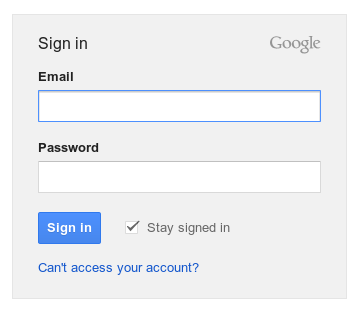
\includegraphics[width=\textwidth]{loginForm.png}
\end{subfigure}%
~
\begin{subfigure}[t]{0.5\textwidth}
\centering
\vspace*{-9.75em}
\begin{listing}
\begin{spverbatim}
<h2>Sign in <strong></strong></h2>
<form novalidate id="gaia_loginform" action="https://accounts.google.com/ServiceLoginAuth" method="post">


<div class="email-div">
  <label for="Email"><strong class="email-label"> Username</strong></label>
  <input type="email" spellcheck="false" name="Email" id="Email" value="">
</div>
  
<div class="passwd-div">
  <label for="Passwd"><strong class="passwd-label"> Password</strong></label>
  <input type="password" name="Passwd" id="Passwd">
</div>
<input type="submit" class="g-button g-button-submit" name="signIn" id="signIn" value="Sign in">
\end{spverbatim}
\end{listing}
\end{subfigure}

\end{figure}

\end{frame}

%\begin{frame}{Password Based Authentication on the Web}{}
%
%	\begin{figure}
%\centering
%\begin{tikzpicture}
%	\node[state, align=left] at (0,-1) {\pgfimage[width=1.5cm]{browser}};
%		
%	\node[state] (client1) at (1.5,-1){};
%	\node[state] (client2) at (1.5,-2){};		
%	
%	\node[state, align=right] at (7,-1) {\pgfimage[width=1.5cm]{web_server}};
%
%	\node[state] (server1) at (4.75,-1) {};
%	\node[state] (server2) at (4.75,-2) {};
%	
%	\draw[pil] (client1) -- node[above] {\texttt{Bob,Pwd}} (server1);
%	\draw[pil] (server2) -- node[above] {\texttt{access/denied}} (client2);
%
%	\node[state, align=left] at (3,0) {\structure{SSL/TLS}};	
%	\node[cylinder, blue, draw,minimum height=1.5cm, minimum width=2cm,aspect=.5, inner xsep=2cm, inner ysep=1cm] at (3,-1.25) {};
%\end{tikzpicture}
%
%\end{figure}
%\end{frame}

\begin{frame}{Password Based Authentication on the Web}{Drawbacks}
	\begin{itemize}
		\item Requires \structure{PKI}
		\item Server receives \structure{passwords in clear}
		\item User has to \structure{remember} passwords \& password-username-server mapping
	\end{itemize}
	\pause 
	\vspace*{2em}	
	
	\setbeamercolor{uppercol}{fg=white,bg=blue}%
	\setbeamercolor{lowercol}{fg=black,bg=lblue}%
	\begin{beamerboxesrounded}[upper=uppercol,lower=lowercol,shadow=true]{\centering }\centering
		...Not the best way to do it...
	\end{beamerboxesrounded}
	
	\pause 
	\vspace*{2em}	
	
	\setbeamercolor{uppercol}{fg=white,bg=blue}%
	\setbeamercolor{lowercol}{fg=black,bg=lblue}%
	\begin{beamerboxesrounded}[upper=uppercol,lower=lowercol,shadow=true]{\centering Better Solution}\centering
		Password Based Authenticated Key Exchange
	\end{beamerboxesrounded}
	
\end{frame}

\subsection{Password Based Authenticated Key Exchange}

\begin{frame}{Password Based Authenticated Key Exchange (PAKE)}{}

	PAKE protocols known since over 20 years\\
	
	\begin{itemize}
		\item Security against Offline Dictionary attacks
		\item Established security models
		\begin{itemize}
			\item Game Based Security Model \cite{Bellare2000}%[BPR 2001]
			\item Universally Composable PAKE \cite{Canetti2005}%[CHKLK 2005]
		\end{itemize}
		\item Many secure protocols known
		\begin{itemize}
			\item Simple password-based encrypted key exchange protocols \cite{Abdalla2005}
			\item Faster and shorter password-authenticated key exchange \cite{Gennaro2008}
			\item Round-Optimal Password-Based Authenticated Key Exchange \cite{Katz2011}
			\item \dots
		\end{itemize}
	\end{itemize}	

\end{frame}

\begin{frame}{PAKE Protocols}{Example: SPAKE}

 SPAKE \cite{Abdalla2005} uses DL-hard group $G$ and public $M,N\in G$; hash function $H$ as random oracle

\begin{figure}
\centering
\begin{tikzpicture}
	\node[state] (client) at (0,0.25) {\pgfimage[width=0.8cm]{os_tux}};
	
	\node[state, align=left] at (0,-1) {$x\rin\ZZ_p, X\gets g^x$\\  $X'\gets X\cdot M^\pwd$};
	\node[state] (client1) at (2,-1){};
	
	\node[state, align=left] at (0,-2) {$K'_A\gets (Y'/N^\pwd)^x$};
	\node[state] (client2) at (2,-2){};	
	
	%\node[state, align=center] at (0,-3) {$K\gets H(A,B,X',Y',K_A,\pwd)$};
	
	
	\node[state] (server) at (6,0.25) {\pgfimage[width=0.8cm]{techie_sailor}};
	
	\node[state, align=right] at (6,-1) {$y\rin\ZZ_p, Y\gets g^y$\\ $Y\gets Y\cdot N^\pwd$};
	\node[state] (server1) at (4,-1) {};
	
	\node[state, align=right] at (6,-2) {$K'_B\gets (X'/M^\pwd)^y$};
	\node[state] (server2) at (4,-2) {};
	
	%\node[state, align=center] at (6,-3) {$K\gets H(A,B,X',Y',K_B,\pwd)$};
	
	\draw[pil] (client1) -- node[above] {$X'$} (server1);
	\draw[pil] (server2) -- node[above] {$Y'$} (client2);
\end{tikzpicture}
%\caption{Encrypted Key Exchange (EKE)}
\label{fig:eke}
\end{figure}
Key derivation:\\
$K_A\gets H(A,B,X',Y',K'_A,\pwd)$\\
$K_B\gets H(A,B,X',Y',K'_B,\pwd)$

\end{frame}

%\begin{frame}{PAKE Protocols}{Advantages}
%
%	Offer appealing properties for Web Authentication
%	\vspace*{2em}
%	
%	\begin{itemize}
%		\item No server certificates (PKI) needed
%		\item Passwords are \structure{not transmitted} at all
%	\end{itemize}	
%
%\end{frame}

\begin{frame}{PAKE on the Web}{}

	\begin{figure}
\centering
\begin{tikzpicture}
	\node[state, align=left] at (-0.5,-2) {\pgfimage[width=2cm]{browser}};
		
	\node[state] (client1) at (1.5,-1){};
%	\node[state] (client2) at (1.5,-2){};
%	\node[state] (client3) at (1.5,-3){};
	\node[state] (client4) at (1.5,-2.5){};
	
	\node[state, align=right] at (7.5,-2) {\pgfimage[width=2cm]{web_server}};

	\node[state] (server1) at (4.75,-1) {};
%	\node[state] (server2) at (4.75,-2) {};
%	\node[state] (server3) at (4.75,-3) {};
	\node[state] (server4) at (4.75,-2.5) {};
	
	\draw[pil,<->] (client1) -- node[above] {\texttt{PAKE}} (server1);
%	\draw[pil] (server2) -- node[above] {$\mathtt{challenge}_K$} (client2);
%	\draw[pil] (client3) -- node[above] {$\mathtt{response}_K$} (server3);

	\node[state, align=left] at (3,-1.5) {\structure{Secured$_K$}};	
	\node[cylinder, blue, draw,minimum height=1.5cm, minimum width=1.5cm,aspect=.5, inner xsep=2cm, inner ysep=0.5cm] at (3,-2.5) {};
	\draw[pil,<->] (client4) -- node[above] {} (server4);
\end{tikzpicture}

\end{figure}

\vspace*{1em}

%	\begin{itemize}
%		\item Establish client -- server connection
%		\item Run PAKE protocol
%		\item Establish secure channel using the exchanged key
%	\end{itemize}
	
	\begin{itemize}
		\item No server certificates (PKI) needed
		\item Passwords are \structure{not transmitted} at all
	\end{itemize}	

\vspace*{1em}

	\structure{However}, PAKE protocols are \structure{hardly used} in practice (missing standards / incompatibility may be a reason)

\end{frame}

\begin{frame}{The Problem of Failed Logins}{}

	Users are still not good with passwords \cite{Florencio2007,Gaw2006a}:
	
	\begin{itemize}
		\item 2.4 failed login attempts on average
		\item 6.5 different passwords in use\\ (on approx. 25 accounts)
		\item \structure{Password disclosure} with current practice
	\end{itemize}
	\pause\vspace*{1em}

	\begin{columns}[t]
    \begin{column}{.475\linewidth}
	    	{\centering\structure{PAKE}}\\
	    	\begin{itemize}
	    		\setlength{\itemindent}{-1em}
	    		\item Run $n$ PAKE protocols
		    \item Linear amount of work
%	    		\item Communication overhead
	    	\end{itemize}
    \end{column}
    \begin{column}{.475\linewidth}
    		{\centering\structure{TLS-based}}\\
    		\begin{itemize}
	    		\setlength{\itemindent}{-1em}
	    		\item Establish 1 TLS channel
	    		\item Send $n$ forms
    		\end{itemize}
    \end{column}
  \end{columns}
	\vspace*{2em}
	SPAKE execution for $3$ passwords: $3\times4$ Exponentiations%, $3\times2$ Multiplications, $3$ Inversions, $3$ Hashes
\end{frame}

\subsection{Goals of this Work}

\begin{frame}{Oblivious PAKE}{}

	\setbeamercolor{uppercol}{fg=white,bg=blue}%
	\setbeamercolor{lowercol}{fg=black,bg=lblue}%
	\begin{beamerboxesrounded}[upper=uppercol,lower=lowercol,shadow=true]{}\centering
		Efficient PAKE with multiple client input passwords
	\end{beamerboxesrounded}

	
	\pause	
	\vspace*{2em}	
	
	\structure{Goals}	
	
	\begin{itemize}
		\item \structure{Efficient} handling of password trials
		\item \structure{No leakage} of non-matching passwords to the server
		\item Ease user's password handling
	\end{itemize}
	
\end{frame}

\section{Oblivious PAKE}

\subsection{Setting}

\begin{frame}{Oblivious PAKE}{Setting}

	\begin{itemize}
		\item Client and server share password $\pwd$
		\item Client inputs a list of up to $c$ passwords $\pwdv$
		\item Server can restrict $c$ due to online dictionary attacks
	\end{itemize}

\centering\structure{Successful iff $\pwd\in\pwdv$}	
\begin{figure}
\centering
\begin{tikzpicture}
	\node[state] (client) at (0,0.5) [align=center]{\pgfimage[width=0.8cm]{os_tux}\\ Client};
	
	\node[state, align=left] at (0,-1) {$\pwdv$,  $|\pwdv|\leq c$};
	\node[state] (client1) at (1.2,-1){};
	\node[state] (client2) at (1.2,-2){};
	
	\node[state] (server) at (6,0.5) [align=center]{\pgfimage[width=0.8cm]{techie_sailor}\\ Server};
	
	\node[state, align=center] at (6,-1) {$\pwd$};
	\node[state] (server1) at (5.6,-1) {};
	\node[state] (server2) at (5.6,-2) {};
	
	\node[state] (middle1) at (3.7,-1.2) {};
	\node[state] (middle2) at (3.7,-1.0) {};

	\node[box] (box) at (3.2,-1)[align=center]{\large O-PAKE};
	
	\draw[pil] (client1) -- (box);
	\draw[pil] (server1) -- (box);
	
	\draw[pil] ($(box.south)-(0.7,0)$) |- node[below] {\hspace*{-2em}$k_C$}(client2);
	\draw[pil] ($(box.south)-(-0.7,0)$) |- node[below] {\hspace*{3em}$k_S$}(server2);
	
	%\draw[pil,<->] (client1) -- node[above] {$\mathrm{PAKE}_{\pwd}$} (server1);
	%\draw[pil] (middle2) edge [loop above, ->,out=70,in=320,distance=1cm] (middle1);
	
\end{tikzpicture}
%\caption{Encrypted Key Exchange (EKE)}
%\label{fig:eke}
\end{figure}		
	
\end{frame}

\begin{frame}{Oblivious PAKE}{Setting}
\begin{figure}
	\includegraphics[width=\textwidth]{impl.png}
\end{figure}
\end{frame}

\begin{frame}{Oblivious PAKE}{Security Model}
	Game based security model from \cite{Bellare2000,Abdalla2005a}: %[BPR 2001, AFP 2005]:
	\begin{itemize}
		\item Real-or-Random (multiple Test queries)
		\item Forward Secrecy (Corrupt oracle)
		\item Extended to allow multiple input passwords
	\end{itemize}
	
	\begin{figure}
		\fbox{
		\begin{tikzpicture}
			\node[state, align=left] at (3,-1) {$c\in\NN, b\rin\bits$\\
				$\forall(P,P')\in\cC\times\cS$, pick $\pwd_{P,P'}\rin\cD$\\
				$b'\gets\cA^{\send,\execute,\corrupt,\test}(\secpar, c)$\\
				return $b\cmp b'$};
		\end{tikzpicture}}
	\end{figure}

\end{frame}

\begin{frame}{Oblivious PAKE}{Na{\"i}ve Solution}

\setblockcolor{blue!10}
\setbordercolor{blue!15}

\begin{dynblock}
% First block
\opaqueblock<1>{\vspace*{-1em}
\begin{figure}
\centering
\includegraphics[width=\textwidth]{npake}
\end{figure}
}
\invblock<2->

% Second block
\opaqueblock<2>[0.6\textwidth]{
Run $c$ sessions of the same PAKE
	\begin{itemize}
		\item \structure{Client:}\\\hspace*{2em}
		linear amount of work
		\item \structure{Server:}\\\hspace*{2em}
		linear amount of work
	\end{itemize}
\vspace*{1em}
Successful iff 1 session successful
}

\end{dynblock}

\end{frame}

% ------------------------------
\newcommand{\drawoverlays}{%
\node[rectangle,draw=black,rounded corners, fill=black!20, text width=5.25em, minimum height=12em] (client) at (2.95,-2.5){}; %draw=black, very thick,
\node[rectangle,draw=black,rounded corners, fill=black!20, text width=5.25em, minimum height=12em] (client) at (6.2,-2.5){};
\node[rectangle,draw=black,rounded corners, fill=black!20, text width=26em, minimum height=2.2em] (client) at (3,-7.1){};
}

\newcommand{\drawoverlay}{%
\node[rectangle,draw=black,rounded corners, fill=black!20, text width=26em, minimum height=2.2em] (client) at (3,-7.1){};
}

\newcommand{\drawopake}[6]{%
\begin{frame}{Oblivious PAKE}{#5}
\begin{figure}
\vspace*{-1em}
\centering
\scalebox{0.8}{%
\begin{tikzpicture}%,text width=0em
	\node[state] at (1,1.2) [align=center]{\pgfimage[width=0.8cm]{os_tux}\\ Client};	
%
	\node[state, align=left] at (-1.5,-1) {$\mathbf{pw}[1]$};
	\node[state, align=left] at (-1.5,-4) {$\mathbf{pw}[c]$};
	\node[state] (client1) at (-1,-1){};
	\node[state] (client2) at (-1,-2.5){};
	\node[state] (client25) at (-1,-4){};
	\node[state] (client3) at (-1,-4.5){};
%	
	\node[state] at (6.5,1.2) [align=center]{\pgfimage[width=0.8cm]{techie_sailor}\\ Server};
%	
	\node[state, align=right] at (8.2,-1) {pw};
	\node[state] (server1) at (8.1,-2.5) {};
	\node[state] (server2) at (8,-1) {};
	\node[state] (server25) at (8.4,-4) {};
	\node[state] (server3) at (8.4,-4.5) {};
%	
	\node[box, text width=3.5em] (box1) at (.5,-1)[align=center]{\large PAKE};
	\node[box, text width=3.5em] (box2) at (.5,-4)[align=center]{\large PAKE};
%	
	\node[bigbox, text width=1.5em] (box3) at (2.25,-2.5)[align=center]{\large #1};
	\node[bigbox, text width=1.5em] (box4) at (3.65,-2.5)[align=center]{\large #2};
	\node[bigbox, text width=1.5em] (box5) at (5.5,-2.5)[align=center]{\large #3};
	\node[bigbox, text width=1.5em] (box52) at (6.9,-2.5)[align=center]{\large #4};
%	
	\node[box, text width=3.5em] (box6) at (7.3,-5.75)[align=center]{\large PAKE};
%	
	\draw[pil] (box1.east) -- node[above] {$m_1$}(box1-|box3.west);
	\draw[pil] (box2.east) -- node[above] {$m_c$}(box2-|box3.west);
	\draw[pil] ([yshift=1.5cm]box3.east) -- ([yshift=1.5cm]box4.west);
	\draw[pil] ([yshift=-1.5cm]box3.east) -- ([yshift=-1.5cm]box4.west);
	\draw[pil] (box4.east) -- (box4-|box5.west);
	\draw[pil] (box5.east) -- (box5-|box52.west);
%	
	\draw[line width = .5mm,circle dotted] ($(client1)-(0.5,0.5)$) -- ($(client2)-(0.5,1)$);
	\draw[line width = .5mm,circle dotted] ($(box1)-(0,0.5)$) -- ($(box2)-(0,-0.5)$);
%	
	\draw[pil] (client1) -- (box1);
	\draw[pil] (client25) -- (box2);
	\draw[pil] (server2) -- (server2-|box5.east); % -- +(0,.7)
	\draw[pil] (box52.east) -| node[right]{$m$}($(box6.north)+(0.5,0)$);
	\draw[pil] ($(server2)+(0.5,0.1)$) |- (box6.east);
%	
	\node[rectangle,draw=black,rounded corners, draw=black, very thick, text width=17em, minimum height=20em] (client) at (1,-3.75){};
	\node[rectangle,draw=black,rounded corners, draw=black, very thick, text width=9.6em, minimum height=20em] (server) at (6.7,-3.75){};
	\node[rectangle,draw=black,rounded corners, draw=black, very thick, text width=16em, minimum height=13em] (clientpake) at (1.05,-2.5){};
%	
	\draw[pil] (box6.west) -| node[below] {$m$}(clientpake.south);
%
	\node[box, text width=6.5em] (box7) at (6.5,-7)[align=center]{\large Confirmation};
	\node[box, text width=8em] (box8) at (0,-7)[align=center]{\large Key Derivation};
%
	\draw[pil] (box6.south) -- node[auto] {$k$}(box6|-box7.north);
	\draw[pil] (box7) -- node[auto] {$k_f$}($(box7)-(0,1.2)$);
	\draw[pil] ([xshift=-1cm]clientpake.south) -- node[left] {$(k_1,\dots,k_c)$}([xshift=-1cm]clientpake|-box8.north);
	\draw[pil] (box7.west) -- node[auto] {conf}(box8.east);
	\draw[pil] (box8) -- node[auto] {$k_f$}($(box8)-(0,1.2)$);
% Gray overlays %
	#6
\end{tikzpicture}}
\end{figure}
\end{frame}
}

\subsection{Idea}

\drawopake{?}{?}{?}{?}{Idea}{\drawoverlays}


\subsection{Building Blocks}

\begin{frame}{Building Blocks}{Index-Hiding Message Encoding (IHME)}

	IHME, introduced in \cite{Manulis2010}, is a message encoding with following properties: %[MPP 2010]
	%\vspace*{1em}
	\begin{itemize}
		\item Encodes set of index, message pairs $(i,m)$
		\item Ensures hiding of index $i$
		\item Length preserving
	\end{itemize}

	\vspace*{1em}

	\setbeamercolor{uppercol}{fg=white,bg=blue!40}%
	\setbeamercolor{lowercol}{fg=black,bg=blue!20}%
	\pause
	\begin{beamerboxesrounded}[upper=uppercol,lower=lowercol,shadow=true]{$S\gets\iencode(P)$}
		$P=\{(\pwdv[1],m_{1}),\dots,(\pwdv[c],m_{c})\}\rightarrow S=(a_{c-1},\dots,a_0)$\\\\
		$f=\sum^{c-1}_{k=0}a_kx^k$ s.t. $f(\pwdv[i])=m_{i}~~\forall(\pwdv[i],m_{i})\in P$
	\end{beamerboxesrounded}
	
	\vspace*{1em}

	\begin{beamerboxesrounded}[upper=uppercol,lower=lowercol,shadow=true]{$m\gets\idecode(S, \pwd)$}
		$(S=(a_{c-1},\dots,a_0), \pwd)\rightarrow m$ with	$m=f(\pwd)$
	\end{beamerboxesrounded}
	
\end{frame}

%\begin{frame}{Building Blocks}{Index-Hiding Message Encoding (IHME)}
%
%	\setbeamercolor{uppercol}{fg=white,bg=blue!40}%
%	\setbeamercolor{lowercol}{fg=black,bg=blue!20}%
%	\begin{beamerboxesrounded}[upper=uppercol,lower=lowercol,shadow=true]{$S\gets\iencode(P)$}
%		$P=\{(\pwdv[1],m_{1}),\dots,(\pwdv[c],m_{c})\}\rightarrow S=(a_{c-1},\dots,a_0)$\\\\
%		$f=\sum^{c-1}_{k=0}a_kx^k$ s.t. $f(\pwdv[i])=m_{i}~~\forall(\pwdv[i],m_{i})\in P$
%	\end{beamerboxesrounded}
%	
%	\vspace*{2em}
%
%	\begin{beamerboxesrounded}[upper=uppercol,lower=lowercol,shadow=true]{$m\gets\idecode(S, \pwd)$}
%		$(S=\sum^{c-1}_{k=0}a_kx^k, \pwd)\rightarrow m$\\\\
%		$m=f(\pwd)$
%	\end{beamerboxesrounded}
%
%
%\end{frame}

\drawopake{?}{\begin{sideways}\alert{IHME.iEncode}\end{sideways}}{\begin{sideways}\alert{IHME.iDecode}\end{sideways}}{?}{IHME}{\drawoverlay}

\begin{frame}{Building Blocks}{Admissible Encodings}
	Admissible Encodings $F:S\rightarrow R, \cI_F:R\rightarrow S$, introduced in \cite{BonehF01,BrierCIMRT10,pseudorandomSignatures} encodes elements from set $S$ to $R$ such that: %[BF 2001, FGKMP 2013]
	\begin{itemize}
		\item $\cI_F(r)$ is statistically indistinguishable from uniform distribution over $S$
		\item Efficient computable
	\end{itemize}
	
	\pause\vspace*{1em}
	%SPAKE uses the following Admissible Encodings to map $G_q\mapsto \ZZ_N$
	
%	\begin{itemize}
%		\item 
		SPAKE uses Admissible Encoding to map arbitrary subgroups $G_q \subseteq \ZZ_N^\ast \mapsto \ZZ_N$ of prime order $q$\\ (cf. ~\cite[Lemma~12]{pseudorandomSignatures}) %p^\times
%		\item Set $R=\{0,\dots,N-1\}=\ZZ_N$ of natural numbers, for arbitrary $N\in\NN$. (cf. ~\cite[Lemma~12]{pseudorandomSignatures})
%	\end{itemize}		
	
\end{frame}

%\begin{frame}{Building Blocks}{Admissible Encodings}
%Further admissible encodings:
%\begin{itemize}
%	\item The set of quadratic residues modulo safe primes~$p$, i.e.\ $R=QR(p)\subseteq\ZZ_p^\times$. (cf. ~\cite[Lemma~12]{pseudorandomSignatures})   
%    \item The set $R=E(\FF)$ of rational points on (certain) elliptic curves, defined over a finite field (cf. ~\cite{BrierCIMRT10}).
%\end{itemize}
%
%\end{frame}

\drawopake{\begin{sideways}\alert{Admissible Encoding$^{-1}$}\end{sideways}}{\begin{sideways}IHME.iEncode\end{sideways}}{\begin{sideways}IHME.iDecode\end{sideways}}{\begin{sideways}\alert{Admissible Encoding}\end{sideways}}{Admissible Encodings}{\drawoverlay}

\drawopake{\begin{sideways}\alert{Admissible Encoding$^{-1}$}\end{sideways}}{\begin{sideways}IHME.iEncode\end{sideways}}{\begin{sideways}IHME.iDecode\end{sideways}}{\begin{sideways}\alert{Admissible Encoding}\end{sideways}}{Key Confirmation}{}

\subsection{O-PAKE Compiler}

\begin{frame}{O-PAKE Compiler}{On the example of SPAKE}
	
\begin{figure}
\centering
\resizebox{\textwidth}{!}{%
\begin{tikzpicture}
	\node[state, align=center, text width=6cm] (client) at (0,1.25) {\pgfimage[width=0.8cm]{os_tux}\\ Client, $\pwdv$};
	
	\node[state, align=left, text width=6cm] at (0,-1) {\setlength{\baselineskip}{20pt}\alert{For $\pwd_i\in\pwdv$}\\\hspace*{1em} $x\rin\ZZ_p, X\gets g^x$\\\hspace*{1em}  $X'_i\gets X\cdot M^{\pwd_i}$\\\hspace*{1em} \alert{$P=P\bigcup(\pwd_i,\cI_F(X'_i))$} \\ \alert{$S\gets$IHME.encode$(P)$}};
	\node[state, text width=6cm] (client1) at (6,-1){};
	
	\node[state, text width=6cm, align=left] at (0,-5) {\setlength{\baselineskip}{20pt}\alert{For $\pwd_i\in\pwdv$}\\\hspace*{1em} $K'_A\gets (Y'/N^\pwd)^x$\\\hspace*{1em} $K_A^i\gets H(A,B,X',Y',K'_A,\pwd)$\\\hspace*{1em}\alert{$C'\gets\PRF_{K_A^i}(S,Y',0)$}\\\hspace*{1em}\alert{IF $C\cmp C'$}\\\hspace*{2em} \alert{$K_{A_F}\gets\PRF_{K_A}(S,Y',1)$}\\\hspace*{2em}\alert{break}};
	\node[state, text width=6cm] (client2) at (0,-3){};
	
	\node[state, text width=6cm] (client3) at (0,-4.5){};
	
	%\node[state, align=center] at (0,-3) {$K\gets H(A,B,X',Y',K_A,\pwd)$};
	
	
	\node[state, text width=6cm, align=center] (server) at (6,1.25) {\pgfimage[width=0.8cm]{techie_sailor}\\ Server, $\pwd$};
	
	\node[state, text width=6cm, align=left] at (7.5,-1) {\setlength{\baselineskip}{20pt}\alert{$X^\ast\gets$IHME.decode$(\pwd,S)$\\ $X'\gets F(X^\ast)$}\\$y\rin\ZZ_p, Y\gets g^y$\\ $Y\gets Y\cdot N^\pwd$};
	\node[state, text width=6cm] (server1) at (7,-1) {};
	
	\node[state, text width=6cm, align=left] at (7.5,-4) {\setlength{\baselineskip}{20pt}$K'_B\gets (X'/M^\pwd)^y$\\ $K_B\gets H(A,B,X',Y',K'_B,\pwd)$\\\alert{$C\gets\PRF_{K_B}(S,Y',0)$}\\\alert{$K_{B_F}\gets\PRF_{K_B}(S,Y',1)$}};
	\node[state, text width=6cm] (server2) at (1,-3) {};
	
	\node[state, text width=6cm] (server3) at (1,-4.5) {};
	
	%\node[state, align=center] at (6,-3) {$K\gets H(A,B,X',Y',K_B,\pwd)$};
	
	\draw[pil] (client1) -- node[above] {\alert{$S$}} (server1);
	\draw[pil] (server2) -- node[above] {$Y'$} (client2);
	\draw[red,pil] (server3) -- node[above] {\alert{$C$}} (client3);
\end{tikzpicture}}
\end{figure}

\end{frame}

\subsection{Implementation \& Performance}

\begin{frame}{OPAKE Implementation}{}
	\structure{Modular} implementation
	\begin{itemize}
		\item Generic Oblivious PAKE Protocol, including
		\begin{itemize}
			\item IHME
			\item Admissible Encodings for $G_q\mapsto\ZZ_N$
		\end{itemize}
	\end{itemize}

	\pause
	\vspace*{2em}
	Implementing an O-PAKE instance includes:
	\begin{itemize}
		\item Implementation of suitable PAKE protocols
		\item Poss. implementation of an admissible encoding
	\end{itemize}
	
\end{frame}

\begin{frame}[fragile]{OPAKE Performance}{Oblivious SPAKE Implementation}
\begin{figure}[tbp]
\centering
%	\begin{subfigure}[b]{0.5\textwidth}
%		\begin{tikzpicture}[scale=0.85]
%		\begin{axis}[xlabel={Number of used Passwords $n$},ylabel={Time [ms]},legend pos= north west,ymax=1200,ymin=0]
%			\addplot+[mark=square,black] table[x index=0,y index=6,col sep=space] {measurements.txt};
%			\addlegendentry{O-RG-PAKE}		
%			\addplot+[mark=triangle,black] table[x index=0,y index=8,col sep=space] {measurements.txt};
%			\addlegendentry{N-RG-PAKE}
%		\end{axis}
%		\end{tikzpicture}
%		%\caption{Oblivious RG-PAKE}
%		%\label{fig:orgpake}
%	\end{subfigure}\hspace*{0.5cm}
%	\begin{subfigure}[b]{0.5\textwidth}
		\begin{tikzpicture}[scale=0.85]
		\begin{axis}[xlabel={Number of used Passwords $n$},ylabel={Time [ms]},legend pos= north west,ymax=50,ymin=0]
			\addplot+[mark=square*] table[x index=0,y index=2,col sep=space] {measurements.txt};
			\addlegendentry{O-SPAKE}
			\addplot+[mark=triangle*] table[x index=0,y index=4,col sep=space] {measurements.txt};
			\addlegendentry{N-SPAKE}
		\end{axis}
		\end{tikzpicture}
		%\caption{Oblivious SPAKE}
		%\label{fig:ospake}
%	\end{subfigure}
%	\caption{Server-side Timings for Oblivious RG-PAKE (left) and SPAKE (right) Protocols}\label{fig:orgpake}
\end{figure}
\end{frame}

\section{Summary}

\begin{frame}{Summary}

  \begin{itemize}
  \item We proposed \alert{Oblivious PAKE} with multiple client passwords
  \item \alert{Constant server runtime} even on failed login attempts
  \item \alert{Modular implementation} of the compiler
  \item Compiler implementation using SPAKE \cite{Abdalla2005} and RG-PAKE \cite{Gennaro2008}
  \end{itemize}
  
  \vskip0pt plus.5fill
  \begin{itemize}
  \item
    Outlook
    \begin{itemize}
    \item Real world application (e.g. browser integration)
    \item Reduce Communication overhead
    \end{itemize}
  \end{itemize}
\end{frame}

\newcommand{\beginbackup}{
   \newcounter{framenumbervorappendix}
   \setcounter{framenumbervorappendix}{\value{framenumber}}
}
\newcommand{\backupend}{
   \addtocounter{framenumbervorappendix}{-\value{framenumber}}
   \addtocounter{framenumber}{\value{framenumbervorappendix}} 
}

\beginbackup
\appendix
\section<presentation>*{\appendixname}
\subsection<presentation>*{References}

\begin{frame}[allowframebreaks]
  \frametitle<presentation>{References}
  \bibliographystyle{alpha}
  \bibliography{references}
\end{frame}
\backupend

\end{document}


